\documentclass[a4paper,11pt]{article}
\usepackage{CJKutf8}
\usepackage{listings}
\usepackage{graphics}
%\DeclareGraphicsExtensions{.pdf,.png,.jpg}
\title{苏州大学 《操作系统 》课程试卷 \\ 试卷}
\date{}
%\date{2012年5月2日}

\begin{document}
\begin{CJK*}{UTF8}{gbsn}

\maketitle

\section{简答与计算}
\subsection{本题共15分}
在某32位机器上, 操作系统进行分页时每个页面大小为4096字节, 采用两级分页技术,其中32位二进制地址中最高10位用于索引第一级页表,
中间10位用于索引第二级页表. 某进程被分配到的虚拟地址空间为第\verb|0x20000000|字节到\verb|0x2007ffff|字节(包括两端点), 
请回答以下问题:
\begin{enumerate}
\item 该进程分配到的虚拟地址空间一共是多少字节? 
\item 这些空间需要多少页面存放? (所有结果以十进制给出)
\item 该进程运行时, 在内存中共需要几张页表? (一级页表和二级页表都考虑在内)
\item 如果仍按照4096字节的页面大小, 则页表规模多大? (以字节计算)
\item 给定地址\verb|0x2ff000f|, 该地址对应一级页表中的第几项? 二级页表中第几项?
\end{enumerate}
注意: 你的答案均需用十进制表示.
\\[3in]


\subsection{本题5分}
假设你作为操作系统设计者, 在设计文件系统时你一般会在你的系统中记录文件的哪些属性? (要求列举不少于4个属性及其作用)
\\[1in]

\subsection{}
在32位PC机上,采用分页技术(只利用一级页表),请回答: \\%如果虚拟内存系统按照4M大小对进程的虚拟地址空间进行分页,请回答:
(a) 如果每页大小为4M,则32位虚拟地址中需要多少位用于描述页内偏移(页内地址)? 多少位用于对页表进行索引?\\
(b) 如果每页大小为4K,且系统实际安装的物理内存大小为1G,则页表项中页框号这个字段至少需要多少个二进制位?
\\[1in]

%\subsection{}
%某进程在某一时刻的页表如下图所示,请计算该进程地址空间中虚拟地址8592所对应的物理地址的值。
%
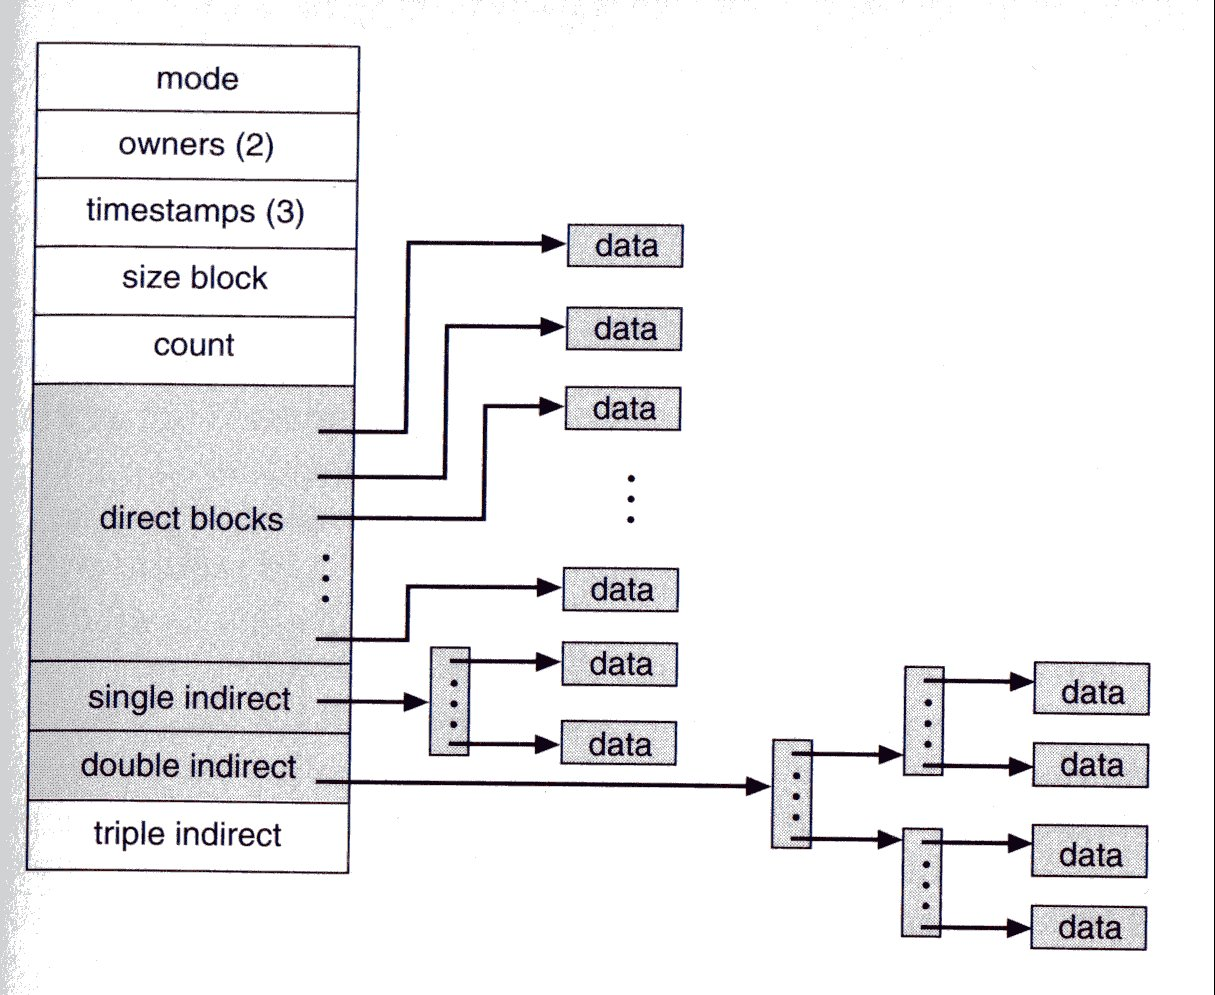
\includegraphics{inode-detail.jpg}
%\\[1in]

\newpage
\subsection{}
在生产者--消费者问题中,分别给出给出以下生产者和消费者程序代码,其中调用了操作系统提供的函数sleep和weakup.
请指出这段代码中存在的竞争条件.

%\lstset{language=C, frame=trbl}
%\lstinputlisting{prodcons.c}
\begin{verbatim}
#define N 100
int count = 0;
int buf[N];

void producer(void) {
    int item;

    while (1) {
        item = produce_item();
        if (count == N) sleep();
        insert_item(item);
        count += 1;
        if (count == 1) wakeup(consumer);
    }
}

void consumer(void) {
    int item;

    while (1) {
        if (count == 0) sleep();
        item = remove_item();
        count -= 1;
        if (count == N-1) wakeup(producer);
        consume_item();
    }
}
\end{verbatim}


\newpage
\subsection{}
阅读以下某机器汇编语言代码,并回答问题:

%\lstset{language=C, frame=trbl}
%\lstinputlisting{tsl.c}
\begin{verbatim}
enter_region:
    TSL REG, LOCK
    CMP REG, #0
    JNE enter_region
    RET

leave_region:
    MOVE LOCK, #0
    RET
\end{verbatim}
\begin{enumerate}
\item 简要说明以上代码中的TSL指令的功能。
\item 用这里定义的enter\_region和leave\_region可以实现进程互斥进入临界区,请说明原因。
\item 用上述方法实现互斥访问临界区的缺点是什么?
\item 在多核处理器上,上述方法实现互斥访问临界区有什么优点(注:考虑sleep和wakeup开销)?
\end{enumerate}

\newpage
\section{Linux系统调用与C语言编程(每题10分,共20分)}

\subsection{}
以下程序的功能是比较两个文件是否相同(省略了头文件和必要的错误检测),但其中两行存在问题,请指出这两行的行号,并给出你对两处错误的修正结果。
%\lstset{language=C, frame=trbl}
%\lstinputlisting{prog2.c}
\begin{verbatim}
int main(int argc,char *argv[])
{
        int fd1,fd2;
        char buff1[1024], buff2[1024];
        int m,n;
        fd1=open(argv[1],O_RDONLY);
        fd2=open(argv[2],O_RDONLY);
        while(1)
        {       
                n=read(fd1,buff1,1024);   
                m=read(fd2,buff2,1024);
                if(strcmp(buff1,buff2)!=0 || n!=m )
                {
                        printf("not the same!\n");
                        return -1;           
                }
                if(n = 0)
                        break;          
        }
        printf("the two files are the same!\n");
        return 0;
}
\end{verbatim}

\newpage
\subsection{}
以下是一个简单的shell程序源代码,它可以执行不带参数和选项的命令(如不能执行用户命令则打印错误信息),并且可以支持
后台进程(用户输入命令以\&结尾),请在划线处补全程序。
\begin{verbatim}
#include <sys/wait.h>
#include <string.h>
#include <stdio.h>
#include <stdlib.h>
#include <unistd.h>
#define MAXLINE 4096

int main(void) {
        char    buf[MAXLINE];   
        pid_t   pid;
        int     status, background;

        printf("%% ");  
        while (fgets(buf, MAXLINE, stdin) != NULL) {
            background = 0;
            if (buf[strlen(buf) - 1] == '\n')
                buf[strlen(buf) - 1] = 0; /* replace newline with null */

            if (buf[strlen(buf) - 1] == '&') {
                ____________________;

                ____________________;
            }
            pid = fork();
            if (pid < 0) 
                exit(1);
            else if (pid == 0) {            /* child */
                execlp(buf, buf, (char *)0);

                ____________________;
                exit(127);
            }
            if ((pid = waitpid(pid, &status, background? WNOHANG : 0)) < 0)
                exit(2);
            printf("%% ");
        }
        exit(0);
}
\end{verbatim}


\section{Linux命令}

\subsection{本题5分}
在线调查脚本程序生成了以下文件\verb|fans.txt|, 其中记录的是每个球迷最喜欢的几位球星的名字, 格式为``球迷姓名 球星1 球星2 ...''.
现在需要用一条命令输出每个球星共有几位球迷喜欢。例如:
\begin{verbatim}
    chenjian 内德韦德 小罗
    chenbing 大罗 C罗 小罗
    luchengtao 
    wangxin 
\end{verbatim}
输出结果为:

\begin{verbatim}
    小罗 2
    大罗 1
    C罗  1
\end{verbatim}
请写出实现该功能的命令。
\\[1in]

\subsection{本题共10分}
文件\verb|scores.txt|记录了某课程学生的平时成绩, 格式为: 

学生姓名\ \ 第1次成绩\ \  第2次成绩\ \ 第3次成绩

\noindent 请写出实现以下功能的命令:
\begin{enumerate}
\item 打印出第三次平时成绩不及格(低于60分)的所有同学的姓名.
\item 如果3次平时成绩的权重分别为0.2, 0.3, 0.5. 请用一条命令输出每位同学的加权平时成绩,格式为`姓名\ \ 加权成绩'.
\end{enumerate}

\subsection{本题5分}
已知当前目录下有7个子目录, 名称分别为lecture1 ... lecture7. 每个目录下均有若干类型的文件(例如PDF, TXT, DOC).
请依次写出以下命令:
\begin{enumerate}
\item 创建名为\verb|all_PDFs|的目录.
\item 将\verb|lecture1| ... \verb|lecture7|目录中所有PDF文件拷贝到目录\verb|all_PDFs|中.
\item 把目录\verb|all_PDFs|打包成名为\verb|all_PDFs.tar|的文件.
\item 把文件\verb|all_PDFs.tar|压缩成文件\verb|all_PDFs.tar.bz2|
\item 如果需要把\verb|all_PDFs.tar.gz2|解压,应该用什么命令?
\end{enumerate}
%\subsection{}

\end{CJK*}
\end{document}

